%% Comandos para los gráficos
\tikzset{
  plot style/.style={
      scale=0.8,
      every node/.style={font={\tiny}},
    },
  nodo/.style 2 args={circle, fill=#1, inner sep=1pt, outer sep=0pt, label={[#1] #2}},
  flecha/.style={dotted, color=#1, -latex},
  eje/.style={-latex, gray, thin},
  ejes/.code={
      \draw[eje] (-1.5,0) -- (3,0) node[below] {$x_0$};
      \draw[eje] (0,-1.5) -- (0,2) node[left] {$x_1$};
    },
}

\begin{enunciado}{\ejercicio}
  Escribir la matriz de las siguientes transformaciones lineales en base canónica.
  Interpretar geométricamente cada transformación.
  \begin{enumerate}[label=(\alph*)]
    \item  $f(x,y) = (x,0) $
    \item  $f(x,y) = (x,-y) $
    \item  $f(x,y) = (\frac{1}{2} (x + y), \frac{1}{2} (x + y))$
    \item  $f(x,y) = (x \cos t - y \sin t, x \sin t + y \cos t) )$
  \end{enumerate}
\end{enunciado}

\begin{enumerate}[label=(\alph*)]
  \item Para la base canónica:
        $$
          f(1,0) = (1,0), \quad f(0,1) = (0,0)
        $$
        Entonces, la matriz asociada es:
        $$
          M =
          \begin{bmatrix}
            1 & 0 \\
            0 & 0
          \end{bmatrix}
        $$
        \begin{minipage}{0.5\textwidth}
          Geométricamente estamos proyectando al eje $x_0$.
        \end{minipage}
        \begin{minipage}{0.5\textwidth}
          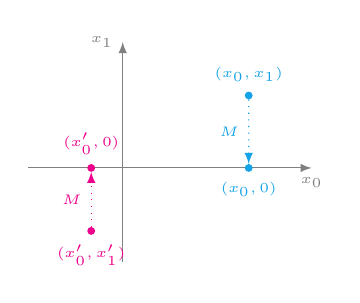
\begin{tikzpicture}[plot style, ejes]
            \node[nodo={Cerulean}{above:{$(x_0,x_1)$}}] (P1a) at (2,1.15) {};
            \node[nodo={Cerulean}{below:{$(x_0,0)$}}] (P1b) at (2, 0) {};
            \draw[flecha={Cerulean}] (P1a) to node[midway, left]{$M$}(P1b) ;

            \node[nodo={magenta}{below:{$(x'_0,x'_1)$}}] (P2a) at (-0.5,-1) {};
            \node[nodo={magenta}{above:{$(x'_0,0)$}}] (P2b) at (-0.5,0) {};
            \draw[flecha={magenta}] (P2a) to node[midway, left]{$M$} (P2b);
          \end{tikzpicture}
        \end{minipage}

        Con el siguiente código vas a poder ver mejor gráficamente el efecto que causa la transformación
        \copyPaste
        \codigoPython{ej-2/codigo2-2-a.py}

  \item Para la base canónica:
        $$
          f(1,0) = (1,0), \quad f(0,1) = (0,-1)
        $$
        Entonces, la matriz asociada es:
        $$
          M =
          \matriz{cc}{
            1 & 0  \\
            0 & -1
          }
        $$
        \begin{minipage}{0.65\textwidth}
          Geométricamente estamos haciendo una reflexión respecto del eje $x_0$.
        \end{minipage}
        \begin{minipage}{0.35\textwidth}
          \begin{tikzpicture}[plot style, ejes]
            \node[nodo={Cerulean}{above:{$(x_0,x_1)$}}] (P1a) at (2,1.5) {};
            \node[nodo={Cerulean}{below:{$(x_0,-x_1)$}}] (P1b) at (2, -1.5) {};
            \draw[flecha={Cerulean}] (P1a) to node[midway, left]{$M$} (P1b);

            \node[nodo={magenta}{below left:{$(x'_0,x'_1)$}}] (P2a) at (-0.5,-1) {};
            \node[nodo={magenta}{above left:{$(x'_0,-x'_1)$}}] (P2b) at (-0.5, 1) {};
            \draw[flecha={magenta}] (P2a) to node[midway, left]{$M$} (P2b);

          \end{tikzpicture}
        \end{minipage}

        Con el siguiente código vas a poder ver mejor gráficamente le efecto que causa la transformación
        \copyPaste
        \codigoPython{ej-2/codigo2-2-b.py}

  \item Para la base canónica:
        $$
          f(1,0) = \left( \frac{1}{2}, \frac{1}{2} \right), \quad f(0,1) = \left( \frac{1}{2}, \frac{1}{2} \right)
        $$
        Entonces, la matriz asociada es:
        $$
          M =
          \begin{bmatrix}
            \frac{1}{2} & \frac{1}{2} \\
            \frac{1}{2} & \frac{1}{2}
          \end{bmatrix}
        $$

        Geométricamente estamos \textit{haciendo, llevando {\tiny (mejores palabras serán bienvenidas)}} todo a la dirección $(1,1)$, ponele.
        $$
          f(x_0,x_1) = \purple{\frac{1}{2}(x_0 + x_1)} \cdot (1,1) \approx \purple{\lambda} \cdot (1,1)
        $$

        Con el siguiente código vas a poder ver mejor gráficamente le efecto que causa la transformación
        \copyPaste
        \codigoPython{ej-2/codigo2-2-c.py}

  \item Para la base canónica:
        $$
          f(1,0) = (\cos t, \sin t), \quad f(0,1) = (-\sin t, \cos t)
        $$
        Entonces, la matriz asociada es:
        $$
          M =
          \begin{bmatrix}
            \cos t & -\sin t \\
            \sin t & \cos t
          \end{bmatrix}
        $$
        \begin{minipage}{0.65\textwidth}
          Geométricamente estamos rotando en sentido antihorario al eje $\ua{x_2}{z}$.
        \end{minipage}
        \begin{minipage}{0.35\textwidth}
          \begin{tikzpicture}[plot style, ejes]
            \node[nodo={Cerulean}{above right:{$(x_0,x_1)$}}] (Pa) at (1,1) {};
            \node[nodo={Cerulean}{below left:{$(x'_0,x'_1)$}}] (Pb) at (-1,-1) {};
            \draw[flecha={Cerulean}] (Pa) arc (45:225:{sqrt(2)}) node[midway, left] {$M_{(t = \pi)}$};
          \end{tikzpicture}
        \end{minipage}
\end{enumerate}

\begin{aportes}
  \item \aporte{https://github.com/juandelia03}{Juan D Elia \github}
  \item \aporte{\dirRepo}{naD GarRaz \github}
\end{aportes}
